\begin{figure}[t]
\centering
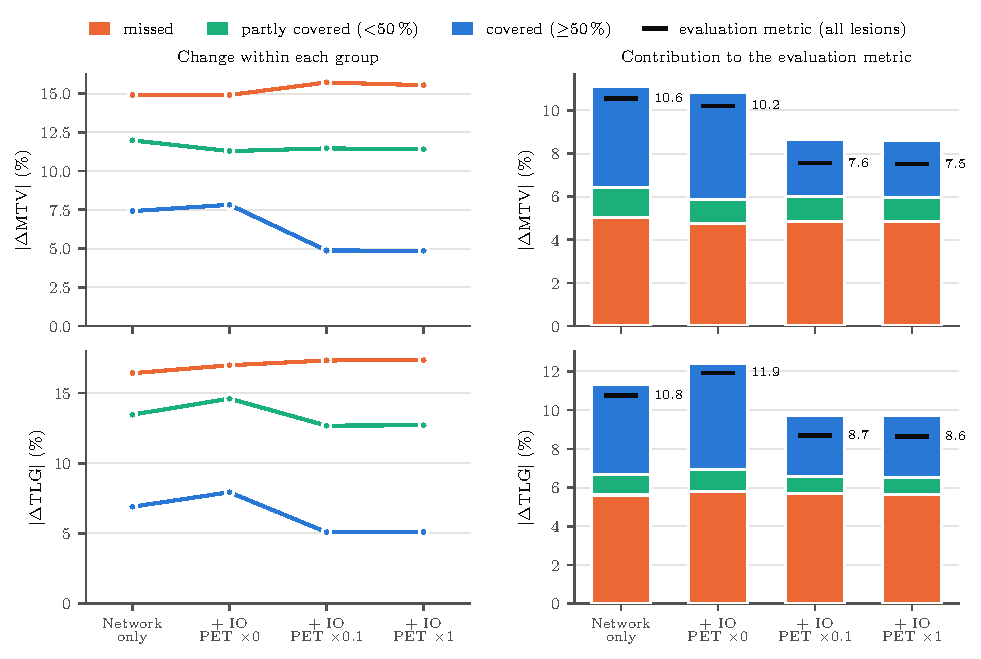
\includegraphics[width=\textwidth]{figures/detection.pdf}
\caption{Registration-induced metabolic tumor volume (MTV) and total lesion glycolysis (TLG) change of all 1435 lesions provided lesion components in 26 test patients (30 pairs), including components smaller than five voxels, grouped by coverage from the predicted lesion mask used by instance optimization (IO): missed (214 lesions, 6\,\% of volume), partly covered (155 lesions, 6\,\% of volume), and covered (1066 lesions, 88\,\% of volume).
The network is trained without PET losses; IO uses the PET weights scaled by the stated factor.
Colors identify coverage groups.
Left: absolute change within each group, computed per image from the group's summed volume or uptake and averaged over patients with lesions in that group; gray dashed: all lesions, the evaluation metric.
Right: contribution of each group to the image-level evaluation metric, averaged over patients; gray ticks show the evaluation metric and lie below the stacked total when opposing lesion changes cancel.}
\label{fig:detection}
\end{figure}
